% Revisione Ready
% Grammatica Ready
% Citazioni Ready

\section{Il problema dell'Hitting Set}\label{sec:il_problema_dell_hitting_set}

Il problema dell'Hitting Set è uno dei pilastri dell'ottimizzazione combinatoria e della teoria della complessità computazionale, noto storicamente per essere uno dei 21 problemi NP-completi di Karp~\cite{karp1972}.
Tale problema riveste una particolare importanza pratica in quanto trova numerose applicazioni in contesti dell'informatica, bioinformatica, data mining e all'interno dei sistemi di diagnostica~\cite{moreno2013, mcguire2014}.
Dal punto di vista teorico, il problema dell'Hitting Set è strettamente correlato al problema noto come \textit{Set Cover}, di cui rappresenta il duale.
Per tale motivo, alcune soluzioni proposte per il Set Cover verranno citate in seguito nell'ambito dei lavori correlati.

\subsection{Definizione formale e varianti}

Sia $U$ un insieme finito, detto universo, e sia $S = \{S_1,S_2,\dots,S_m\}$ una famiglia di sottoinsiemi di U.
Un sottoinsieme $H \subseteq U$ è definito \textit{Hitting Set} per $S$ se interseca ogni sottoinsieme appartenente a $S$, ovvero se
\[
    \forall S_i \in S,\space H \cap S_i \neq \emptyset.
\]
In altre parole, ogni sottoinsieme della collezione, nel nostro caso dunque ogni iperarco, deve contenere almeno un elemento appartenente ad $H$~\cite{garey1979, bretto2013}.
La condizione che rende però tale problema computazionalmente complesso da risolvere non risiede nella difficoltà che si può incontrare nel trovare uno di questi sottoinsiemi, bensì in quella di trovare il sottoinsieme con cardinalità minima che rispetti le proprietà precedentemente citate.

\begin{figure}[h]
    \centering
    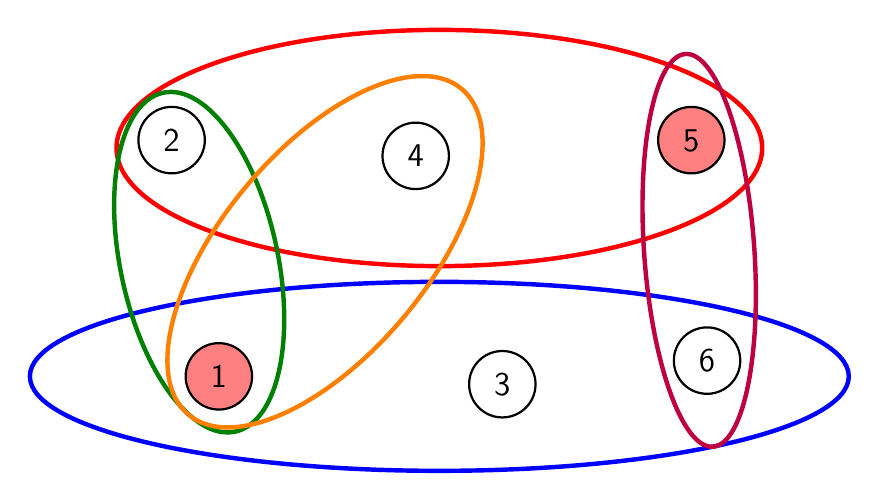
\begin{tikzpicture}[
        % Stile per i nodi standard (bianchi)
        element/.style={circle, draw=black, fill=white, font=\large\sffamily, minimum size=24pt, inner sep=0pt, thick},
        % Stile per i nodi selezionati nel hitting set (rossi)
        hit/.style={element, fill=red!50}
    ]

        % --- COORDINATE DEI NODI ---
        \node[hit]     (N1) at (0.9, 0.2) {1};
        \node[element] (N2) at (0.3, 3.2) {2};
        \node[element] (N3) at (4.5, 0.1) {3};
        \node[element] (N4) at (3.4, 3) {4};
        \node[hit]     (N5) at (6.9, 3.2) {5};
        \node[element] (N6) at (7.1, 0.4) {6};

        % --- INSIEMI (ELLISSI) ---
        
        % Insieme Blu (Orizzontale in basso)
        \draw[blue, ultra thick] (3.7, 0.2) ellipse (5.2cm and 1.2cm);
        
        % Insieme Rosso (Orizzontale in alto)
        \draw[red, ultra thick] (3.7, 3.1) ellipse (4.1cm and 1.5cm);
        
        % Insieme Verde (Inclinato a sinistra, unisce 1 e 2)
        \draw[green!50!black, ultra thick, rotate around={12:(0.65,1.65)}] (0.65, 1.65) ellipse (1.0cm and 2.2cm);
        
        % Insieme Arancione (Inclinato al centro, unisce 1 4)
        \draw[orange, ultra thick, rotate around={-40:(2.3,2)}] (2.4, 1.8) ellipse (1.3cm and 2.7cm);
        
        % Insieme Viola (Verticale a destra, unisce 5 e 6)
        \draw[purple, ultra thick, rotate around={4:(7.0,1.8)}] (7.0, 1.8) ellipse (0.7cm and 2.5cm);

    \end{tikzpicture}

    \caption{Esempio di Hitting Set in un ipergrafo.}\label{fig:hitting_set}
\end{figure}

Da ora in avanti risulterà inoltre importante distinguere tra hitting set minimale (o Minimal Hitting Set) e hitting set di cardinalità minima (da ora in poi citato come Minimum Hitting Set o MHS): un hitting set minimo è necessariamente minimale, ma non viceversa.
Tale puntualizzazione è importante in quanto il problema di trovare un hitting set di cardinalità minima è NP-hard, mentre l'enumerazione di tutti i Minimal Hitting Set è un problema la cui complessità è legata alla struttura dell'ipergrafo.
All'interno dell'ambiente accademico sono state analizzate diverse varianti del problema, di seguito riporto le più discusse~\cite{gainer2017}:
\begin{itemize}
    \item \textbf{Offline Hitting Set}: variante classica del problema nella quale l'intera famiglia di insiemi è nota a priori e rimane invariata durante l'esecuzione dell'algoritmo.
    \item \textbf{Weighted Hitting Set}: variante nella quale ciascun elemento dell'universo ha un peso o un costo associato; l'obiettivo consiste nel determinare un hitting set che minimizzi il costo totale anziché la sola cardinalità.
    \item \textbf{$k$-Hitting Set}: variante in cui la cardinalità di ciascun insieme della collezione è limitata superiormente da una costante $k$.
    \item \textbf{Enumeration of Minimal Hitting Sets}: variante che richiede la generazione di tutti gli hitting set minimali della famiglia di insiemi considerata.
    \item \textbf{Dynamic Hitting Set}: variante che permette alla collezione di insiemi di venire modificata nel tempo attraverso operazioni di inserimento e rimozione, rendendo necessario l'aggiornamento delle soluzioni calcolate.
    \item \textbf{Online Hitting Set}: variante che permette alla collezione di insiemi di venire modificata progressivamente e che obbliga a prendere decisioni senza la possibilità di conoscere gli input futuri.
\end{itemize}
Tra le varianti sopra elencate, particolare attenzione sarà riservata a quelle che introducono una dimensione temporale nella gestione dell’Hitting Set, vale a dire le varianti offline, dinamica e online, che rappresentano il principale oggetto di studio del presente lavoro.

\subsection{Complessità computazionale}

La natura computazionale dell'Hitting Set è intrinsecamente complessa. Nella celebre opera di Richard Karp del 1972, il problema dell'Hitting Set venne inserito tra i 21 problemi originari dimostrati NP-completi (nella sua versione decisionale)~\cite{karp1972}. Di conseguenza, la variante di ottimizzazione (MHS) appartiene alla classe di complessità NP-hard.
Le implicazioni di questa classificazione sulla letteratura scientifica sono profonde: sotto l'ipotesi $P \neq NP$, il Minimum Hitting Set (MHS) non può essere approssimato in tempo polinomiale entro un fattore logaritmico rispetto alla dimensione dell'universo~\cite{johnson1974, feige1998}.
Per definire il tutto più formalmente, il problema non è approssimabile entro un fattore $(1-o(1))\ln m$, dove $m = |S|$~\cite{feige1998}.
A causa dell'intrattabilità nel caso pessimo di questo problema, la ricerca si è focalizzata sullo sviluppo di algoritmi euristici, algoritmi parametrizzati e su modelli temporali in grado di aggiornare le soluzioni sfruttando la coerenza durante lo sviluppo dei dati senza dover rieseguire il calcolo da zero~\cite{downey2013}.